\subsection{Coequalizer of the projections of a fibered square}

Let X and Y be topological spaces, and let f be a continuous map from X to Y. Denote by Z the fibered square \(X \times_{Y} X\) and by \(p_{1}\) , \(p_{2}\) the two projections from Z to X. We denote by W the fibered product \(X \times_{Y} X \times_{Y} X\) ; for every pair \((s, t)\) of elements of \(\{1,2,3\}\) , we denote by \(q_{st}: W \to Z\) the map defined by \(q_{st}(x_{1}, x_{2}, x_{3}) = (x_{s}, x_{t})\) .

Denote by \(\operatorname{Coeg}(f)\) the groupoid \(\operatorname{Coeg}(\varpi(p_{1}),\varpi(p_{2}))\) , the coequalizer of the two morphisms \(\varpi(p_{1})\) , \(\varpi(p_{2})\) from the Poincaré groupoid \(\varpi(Z)\) into the Poincaré groupoid \(\varpi(X)\) . Denote by \(\gamma\colon\varpi(X)\to\operatorname{Coeg}(f)\) the canonical groupoid morphism. Since \(f\circ p_{1}=f\circ p_{2}\) , the groupoid morphisms \(\varpi(f)\circ\varpi(p_{1})\) and \(\varpi(f)\circ\varpi(p_{2})\) from \(\varpi(Z)\) into \(\varpi(Y)\) are equal; there therefore exists a unique groupoid morphism \(\varpi'(f)\colon\operatorname{Coeg}(f)\to\varpi(Y)\) such that \(\varpi'(f)\circ\gamma=\varpi(f)\) .

DEFINITION 1. --- We say that the map f satisfies property (VK) if it is strict, surjective, and if the morphism \(\varpi'(f)\) is an isomorphism.

Example 1. --- This property holds under one of the following hypotheses:

\begin{enumerate}
\def\labelenumi{(\roman{enumi})}
\item
  The spaces X and Y are delaceable, the space \(X \times_{Y} X\) is locally path-connected, the map f is surjective, proper, separated, with locally connected fibers;
\item
  The spaces X and Y are delaceable, the map f is surjective, proper, separated, with finite fibers, the diagonal \(\Delta_{X}\) of \(X \times_{Y} X\) is open and its complement is locally connected;
\item
  The spaces X and Y are delaceable, the map f is surjective, open, and has the path-lifting property;
\item
  Every point of Y has a neighborhood above which there exists a continuous section of the map f.
\end{enumerate}

Indeed, under each of these hypotheses, the map \(f\) is surjective; it is also strict by virtue of I, p. 18, example 2. Finally, the morphism \(\varpi'(f)\) is an isomorphism, whether under hypotheses (i), (ii), or (iii) according to IV, p. 398, th. 1, or under hypothesis (iv) (IV, p. 400, th. 2).

Proposition 5 of II, p. 208 describes the isotropy groups of the groupoid Coeg(f). The aim of this section is to make explicit, when f satisfies property (VK), the description of the Poincaré groups of Y that follows from it by composition with the groupoid isomorphism \(\varpi'(f)\). The following numbers will be devoted to important special cases.

Suppose that the map f satisfies property (VK).

Let us set \(\mathsf{I} = \pi_0(\mathrm{X})\) , \(\mathsf{J} = \pi_0(\mathrm{Z})\) , \(\mathsf{K} = \pi_0(\mathrm{W})\) ; for \(j \in \mathsf{J}\) and \(s \in \{1,2\}\) we set \(i_s(j) = \pi_0(p_s)(j)\) ; for \(k \in \mathsf{K}\) and \(s\) , \(t \in \{1,2,3\}\) we set \(j_{st}(k) = \pi_0(q_{st})(k)\) . Denote by \(\Gamma\) the frame of the pair \((\varpi(p_1), \varpi(p_2))\) of groupoid morphisms from \(\varpi(\mathrm{Z})\) into \(\varpi(\mathrm{X})\) (II, p. 185, def. 3). This is the quiver \((\mathsf{I}, \mathsf{J}, \pi_0(p_1), \pi_0(p_2))\) , for the orbits of the Poincaré groupoid of a topological space are the path-connected components of that space.

Suppose moreover that Y is path-connected and nonempty. By II, p. 200, remark 2, \(\pi_0(\Gamma)\) is then in bijection with the set of orbits of the groupoid Coeg(f); since the map \(f\) satisfies property (VK), the groupoid Coeg(f) is isomorphic to the groupoid \(\varpi(Y)\) . The graph \(\Gamma\) is thus connected and nonempty.

Let us call the van Kampen data of f the data consisting of the following elements:

\begin{enumerate}
\def\labelenumi{(\roman{enumi})}
\item
  for all \(i \in \mathsf{I}\) a point \(\mathsf{a}(i)\) of the path-connected component \(i\) of \(\mathbf{X}\) ;
\item
  for all \(j \in J\) a point \(\mathsf{b}(j) = (\mathsf{b}_{1}(j), \mathsf{b}_{2}(j))\) of the path-connected component j of Z;
\item
  for all \(k \in \mathsf{K}\) a point \(\mathsf{c}(k) = (\mathsf{c}_1(k), \mathsf{c}_2(k), \mathsf{c}_3(k))\) of the path-connected component \(k\) of \(\mathbf{W}\) ;
\item
  for all \(j \in J\) the class \(\beta_{1}(j)\) of a path in X connecting \(\mathsf{b}_{1}(j)\) to \(\mathsf{a}(i_{1}(j))\) and the class \(\beta_{2}(j)\) of a path in X connecting \(\mathsf{b}_{2}(j)\) to \(\mathsf{a}(i_{2}(j))\) ;
\item
  for all \(k \in K\) and for every pair \((s, t)\) equal to \((1, 2)\) , \((2, 3)\) or \((1, 3)\) the class \(\gamma_{st}(k)\) of a path in Z connecting \((\mathsf{c}_{s}(k), \mathsf{c}_{t}(k))\) to \(\mathsf{b}(j_{st}(k))\) ;
\item
  a subquiver \(\mathsf{T}\) of \(\Gamma\) whose associated graph is a maximal tree of the graph \(\widetilde{\Gamma}\) ;
\item
  an element \(i_{0}\) of \(\mathsf{I}\) .
\end{enumerate}

Let us choose a van Kampen datum of \(f\) . Then, \((\mathsf{a},\mathsf{b},\beta_{1},\beta_{2},\mathsf{T},i_{0})\) is a basic datum of the pair \((\varpi(p_{1}),\varpi(p_{2}))\) of groupoid morphisms from \(\varpi(\mathrm{Z})\) on \(\varpi(\mathrm{X})\) (II, p. 192, def. 4). Moreover, the triples

\[
\mathsf {z} = \left(\left(q _ {1 2} (\mathsf {c} (k)), 1\right), \left(q _ {2 3} (\mathsf {c} (k)), 1\right), \left(q _ {1 3} (\mathsf {c} (k)), - 1\right)\right)
\]

and the path classes \((\gamma_{1,2}(k), \gamma_{2,3}(k), \gamma_{1,3}(k))\) , where k ranges over K, define a complementary equipment of the pair \((\varpi(p_{1}), \varpi(p_{2}))\) (II, p. 208, def. 3; II, p. 205, example; II, p. 205, remark). We shall say that the complete equipment of the coequalizer Coeg(f) thus defined is deduced from the van Kampen datum of f that we have chosen.

For every \(j \in J\) , denote by \(\varphi_{j} \colon \pi_{1}(Z, \mathsf{b}(j)) \to \pi_{1}(X, \mathsf{a}(i_{1}(j)))\) and \(\psi_{j} \colon \pi_{1}(Z, \mathsf{b}(j)) \to \pi_{1}(X, \mathsf{a}(i_{2}(j)))\) the group homomorphisms defined by

\[
\varphi_ {j} = \operatorname{Int} (\beta_ {1} (j)) ^ {- 1} \circ (p _ {1}) _ {*}, \quad v \mapsto \beta_ {1} (j) ^ {- 1} ((p _ {1}) _ {*} (v)) \beta_ {1} (j)\tag{1}
\]

\[
\psi_ {j} = \mathrm{Int} (\beta_ {2} (j)) ^ {- 1} \circ (p _ {2}) _ {*}, \quad v \mapsto \beta_ {2} (j) ^ {- 1} ((p _ {2}) _ {*} (v)) \beta_ {2} (j),
\]

for \(v \in \pi_1(\mathbf{Z}, \mathfrak{b}(j))\) . For all \(k \in \mathsf{K}\) and every \(s \in \{1,2,3\}\) , denote by \(\lambda_s(k)\) the loop class at the point \(\mathfrak{a}(i_s(k))\) in X defined by

\[
\lambda_ {1} (k) = \beta_ {1} (j _ {1 3} (k)) ^ {- 1} \cdot ((p _ {1}) _ {*} (\gamma_ {1 3} (k))) ^ {- 1} \cdot ((p _ {1}) _ {*} (\gamma_ {1 2} (k))) \cdot \beta_ {1} (j _ {1 2} (k)),\tag{2}
\]

\[
\lambda_ {2} (k) = \beta_ {2} (j _ {1 2} (k)) ^ {- 1} \cdot ((p _ {2}) _ {*} (\gamma_ {1 2} (k))) ^ {- 1} \cdot ((p _ {1}) _ {*} (\gamma_ {2 3} (k))) \cdot \beta_ {1} (j _ {2 3} (k)),
\]

\[
\lambda_ {3} (k) = \beta_ {2} (j _ {2 3} (k)) ^ {- 1} \cdot ((p _ {2}) _ {*} (\gamma_ {2 3} (k))) ^ {- 1} \cdot ((p _ {2}) _ {*} (\gamma_ {1 3} (k))) \cdot \beta_ {2} (j _ {1 3} (k)).
\]

Denote by \(\tau\) the unique morphism of groupoids from Grp \((\Gamma)\) into \(\varpi(\mathrm{Y})\) such that the map Som \((\tau)\) maps \(i \in \mathsf{I}\) to \(f(\mathsf{a}(i))\) and Fl \((\tau)\) maps \(j \in \mathsf{J}\) to the class of paths \(f_{*}(\beta_{1}(j))^{-1}f_{*}(\beta_{2}(j))\) connecting \(f(\mathsf{a}(i_{1}(j)))\)

\pandocbounded{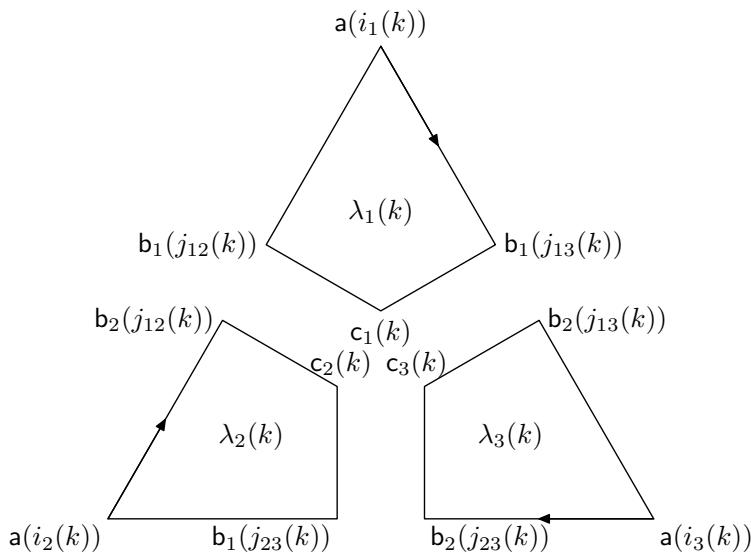
\includegraphics[keepaspectratio]{images/part003_b82e0de6.jpg}}

to \(f(\mathsf{a}(i_2(j)))\) in Y. For \(i \in \mathsf{I}\) , let \(d_i \in \mathrm{Grp}(\Gamma)\) be the class of the unique path without backtracking joining \(i_0\) to \(i\) in the tree \(\widetilde{\mathsf{T}}\) and let us set \(\delta_i = \tau(d_i)\) .

If S is a set, recall that F(S) denotes the free group on S; the image in F(S) of an element \(s \in S\) under the canonical map is denoted {[}s{]}, or even s if there is no possible confusion.

THEOREM 1. --- Suppose that Y is path-connected and that f satisfies property (VK). With the previous notation, there exists a unique group homomorphism

\[
\mathsf {L} \colon \big (\underset {i \in \mathsf {I}} {\ast} \pi_ {1} (\mathrm{X}, \mathsf {a} (i)) \big) \ast \mathrm{F} (\mathrm{J}) \to \pi_ {1} (\mathrm{Y}, f (\mathsf {a} (i _ {0})))
\]

such that

\[
\begin{array}{l l} \mathsf {L} (v) = \delta_ {i} f _ {*} (v) \delta_ {i} ^ {- 1} & \text {for } i\in I \text { and } v\in\pi_{1} (X,a(i)), \\ \mathsf {L} (j) = \delta_ {i _ {1} (j)} \tau (j) \delta_ {i _ {2} (j)} ^ {- 1} & \text {for } j\in J. \end{array}
\]

Moreover, the homomorphism L is surjective and its kernel is the smallest normal subgroup containing the following elements:

\[
\left(\mathrm{R} _ {1}\right) \quad \mathrm{r} _ {1} (j) = j \quad \text {for } j \text { in } \operatorname{Fl} (\mathsf {T});
\]

\[
\left(\mathrm{R} _ {2}\right) \quad \mathfrak {r} _ {2} (j, v) = \varphi_ {j} (v) j \psi_ {j} (v) ^ {- 1} j ^ {- 1} \quad \text {for } j \in \mathsf {J} \text { and } v \in \pi_ {1} (\mathrm{Z}, \mathfrak {b} (j));
\]

\[
\left(\mathrm{R} _ {3}\right) \quad \mathrm{r} _ {3} (k) = \lambda_ {1} (k) j _ {1 2} (k) \lambda_ {2} (k) j _ {2 3} (k) \lambda_ {3} (k) j _ {1 3} (k) ^ {- 1}, \quad \text {for } k \in \mathsf {K}.
\]

The existence and uniqueness of the homomorphism L follow from the universal property of free products and free groups. Moreover, this homomorphism is the composite of the homomorphism \(\varpi'(f)_{\gamma(\mathsf{a}(i_0))}\) deduced from \(\varpi'(f)\) by passing to isotropy groups and to the group homomorphism \(\lambda\) defined by prop. 5 of II, p. 208, taking into account that the chosen van Kampen datum determines a complete equipment of the pair \((\varpi(p_1), \varpi(p_2))\) of groupoid morphisms from \(\varpi(\mathrm{Z})\) into \(\varpi(\mathrm{X})\) . By this proposition, the homomorphism \(\lambda\) has as image the group \(\operatorname{Coeg}(f)_{\gamma(\mathsf{a}(i_0))}\) and its kernel is the smallest normal subgroup containing the elements defined by the relations \((\mathrm{R}_1)\) , \((\mathrm{R}_2)\) and \((\mathrm{R}_3)\) . On the other hand, the groupoid morphism \(\varpi'(f)\) : \(\operatorname{Coeg}(f) \to \varpi(\mathrm{Y})\) is an isomorphism, by definition of property (VK). The theorem is therefore proved.

